\documentclass[a4paper]{article}

\usepackage{inputenc}
\usepackage[british,UKenglish]{babel}
\usepackage{amsmath}
%\usepackage{titlesec}
\usepackage{color}
\usepackage{graphicx}
\usepackage{fancyref}
\usepackage{hyperref}
\usepackage{float}
\usepackage{scrextend}
\usepackage{setspace}
\usepackage{xargs}
\usepackage{multicol}
\usepackage{nameref}

\usepackage{sectsty}
\usepackage{multicol}
\usepackage{multirow}
\usepackage[procnames]{listings}
\usepackage{appendix}

\newcommand\tab[1][1cm]{\hspace*{#1}}
\hypersetup{colorlinks=true, linkcolor=black}
\interfootnotelinepenalty=10000

\newcommand{\cleancode}[1]{\begin{addmargin}[3em]{3em}\texttt{\textcolor{cleanOrange}{#1}}\end{addmargin}}
\newcommand{\cleanstyle}[1]{\text{\textcolor{cleanOrange}{\texttt{#1}}}}


\usepackage[colorinlistoftodos,prependcaption,textsize=footnotesize]{todonotes}
\newcommandx{\commred}[2][1=]{\textcolor{Red}
{\todo[linecolor=red,backgroundcolor=red!25,bordercolor=red,#1]{#2}}}
\newcommandx{\commblue}[2][1=]{\textcolor{Blue}
{\todo[linecolor=blue,backgroundcolor=blue!25,bordercolor=blue,#1]{#2}}}
\newcommandx{\commgreen}[2][1=]{\textcolor{OliveGreen}{\todo[linecolor=OliveGreen,backgroundcolor=OliveGreen!25,bordercolor=OliveGreen,#1]{#2}}}
\newcommandx{\commpurp}[2][1=]{\textcolor{Plum}{\todo[linecolor=Plum,backgroundcolor=Plum!25,bordercolor=Plum,#1]{#2}}}

\def\code#1{{\tt #1}}

\def\note#1{\noindent{\bf [Note: #1]}}

\makeatletter
%% The "\@seccntformat" command is an auxiliary command
%% (see pp. 26f. of 'The LaTeX Companion,' 2nd. ed.)
\def\@seccntformat#1{\@ifundefined{#1@cntformat}%
   {\csname the#1\endcsname\quad}  % default
   {\csname #1@cntformat\endcsname}% enable individual control
}
\let\oldappendix\appendix %% save current definition of \appendix
\renewcommand\appendix{%
    \oldappendix
    \newcommand{\section@cntformat}{\appendixname~\thesection\quad}
}
\makeatother


% "define" Scala
\usepackage[T1]{fontenc}  
\usepackage[scaled=0.82]{beramono}  
\usepackage{microtype} 

\sbox0{\small\ttfamily A}
\edef\mybasewidth{\the\wd0 }

\lstdefinelanguage{scala}{
  morekeywords={abstract,case,catch,class,def,%
    do,else,extends,false,final,finally,%
    for,if,implicit,import,match,mixin,%
    new,null,object,override,package,%
    private,protected,requires,return,sealed,%
    super,this,throw,trait,true,try,%
    type,val,var,while,with,yield},
  sensitive=true,
  morecomment=[l]{//},
  morecomment=[n]{/*}{*/},
  morestring=[b]",
  morestring=[b]',
  morestring=[b]"""
}

\usepackage{color}
\definecolor{dkgreen}{rgb}{0,0.6,0}
\definecolor{gray}{rgb}{0.5,0.5,0.5}
\definecolor{mauve}{rgb}{0.58,0,0.82}

% Default settings for code listings
\lstset{frame=tb,
  language=scala,
  aboveskip=3mm,
  belowskip=3mm,
  showstringspaces=false,
  columns=fixed, % basewidth=\mybasewidth,
  basicstyle={\small\ttfamily},
  numbers=none,
  numberstyle=\footnotesize\color{gray},
  % identifierstyle=\color{red},
  keywordstyle=\color{blue},
  commentstyle=\color{dkgreen},
  stringstyle=\color{mauve},
  frame=single,
  breaklines=true,
  breakatwhitespace=true,
  procnamekeys={def, val, var, class, trait, object, extends},
  procnamestyle=\ttfamily\color{red},
  tabsize=2
}

\lstnewenvironment{scala}[1][]
{\lstset{language=scala,#1}}
{}
\lstnewenvironment{cpp}[1][]
{\lstset{language=C++,#1}}
{}
\lstnewenvironment{bash}[1][]
{\lstset{language=bash,#1}}
{}
\lstnewenvironment{verilog}[1][]
{\lstset{language=verilog,#1}}
{}



\lstset{frame=,basicstyle={\footnotesize\ttfamily}}



\graphicspath{ {images/} }
\usepackage{ctex}
\usepackage{verbatim}
\usepackage{geometry}
\usepackage{amsmath}
\usepackage{pifont}%\ding{192} \ding{172}
\usepackage{tikz}
\usepackage{float}
\usepackage{booktabs}
\usepackage{bm}
\usepackage{siunitx}
\usepackage{enumerate}
%\geometry{a4paper, scale=0.72}
\geometry{a4paper,left=2.5cm,right=2.5cm,top=2.5cm,bottom=2.5cm}
%%%%%%%%%%%%%%%%%%%%%%%%%%%%%%%%%%%%%%%% BEGIN DOC %%%%%%%%%%%%%%%%%%%%%%%%%%%%%%%%%%%%%%%%

\begin{document}
\renewcommand{\contentsname}{目\ 录}
\renewcommand{\appendixname}{附录}
\renewcommand{\appendixpagename}{附录}
\renewcommand{\refname}{参考文献} 
\renewcommand{\figurename}{图}
\renewcommand{\tablename}{表}
\renewcommand{\today}{\number\year 年 \number\month 月 \number\day 日}
\newcommand{\refeq}[1]{\textbf{Eq.(\ref{#1})}}
\newcommand*{\circled}[1]{\lower.7ex\hbox{\tikz\draw (0pt, 0pt)%
    circle (.5em) node {\makebox[1em][c]{\small #1}};}}
    
\title{{\Huge 近代物理实验报告{\large\linebreak\\}}{\Large 实验4-1:\ 高压强电离真空计的校准\linebreak\linebreak}}
%please write your name, Student #, and Class # in Authors, student ID, and class # respectively
\author{\\姓\ 名:付\ 大\ 为\\
学\ 号: 1800011105\\
邮\ 箱: \url{fudw@pku.edu.cn}\\
%班\ 号: xxxxx\\\\
近代物理实验 (II)\\
(2022,春季学期)\\\\
北京大学\\
物理学院\\
2018级1班}
\date{\today}
\maketitle
\newpage

%%%%%%%%%%%%%%%%%%%%%%%%%%%%%%%%%%%%%%%% ABSTRACT %%%%%%%%%%%%%%%%%%%%%%%%%%%%%%%%%%%%%%%%
\begin{center}
{\Large\bf{摘\ 要\\}}
\end{center}

“真空”泛指低于一个大气压的气体充满的空间状态.当前各种真空泵,包括获得超高真空的新型泵大致可分为两类:一类称为“外排”型,即真空泵将气体排出泵体之外,如旋片泵、扩散泵、分子泵等;另一类称为“内吸泵”,即真空泵在一封闭系统中,气体吸附在泵体之内(吸附在某一固体表面上),如吸附泵,钛升华泵、溅射离子泵、冷凝泵等.电离真空计的测量下限是由离子收集电流中的软X射线光电本底电流所决定的.本实验利用膨胀法校准高压强电离真空计,以得到待校准仪表读数与标准仪表读数间的对应关系.
\\\\
{\bf{关键词}:}\ 真空,真空泵,电离真空计,仪器校准

%%%%%%%%%%%%%%%%%%%%%%%%%%%%%%%%%%%%%%%% CONTENT %%%%%%%%%%%%%%%%%%%%%%%%%%%%%%%%%%%%%%%%
\newpage
\begin{center}
\tableofcontents\label{c}
\end{center}
\newpage

%%%%%%%%%%%%%%%%%%%%%%%%%%%%%%%%%%%%%%%% Introduction %%%%%%%%%%%%%%%%%%%%%%%%%%%%%%%%%%%%%%%%
\section{引言} \label{overview}%------------------------------
在电离真空计中,阴极发射的电子被阳极栅(相对阴极为正100$\sim$150V)加速后具有一定能量与气体分子作电离碰撞,使气体电离.所产生的正离子被外围圆筒形离子收集极(相对阴极为负10~60V)收集,在其“线性指示范围”内工作是应该有离子流$I_+$和电子流$I_-$之比与压强p成正比.挡压强升高到电子平均自由程小于电极间电子的平均露出时,平均每个电子有可能碰撞两个或更多的气体分子,此时上述正比关系可能不再成立:离子流首先因离子繁殖而偏大,以后由于电子与分子碰撞过于频繁以致在运动过程中不能从电场中获得足够能量以电离气体,只能作弹性碰撞,所以离子流又逐渐偏小直至最后趋于零.

为了提高测量线性测量上限,可以采取改变电极结构使电子路程缩短的办法,阴极至板状阳极的距离可减小到约1.5mm.它可以在更高的压强下才发生上述电子繁流的现象.改进后的高压强电离真空规可在$10^{-1}\sim10^{-5}\si{Torr}$量程内保持线性指示.

一对平行板作为离子收集极C,中间阴极K与右侧杆状阳极A相距约1.3mm,两外侧为杆状辅助电极S.它的特点是除了缩短电子路径(由K到A),还可因C和S极加上相对阳极为负的电压而增强靠近A极的电场强度E,使得电子在自由程很短的情况下仍可由电场得到足以电离气体的能量,故压强上限可进一步提高.

在测量高真空时,为了降低测量下限,将离子收集极上的负电压减小并把S极作为加速阳极使用,这样的安排使电子在更大的空间区域有较高的动能,因而提高了测量灵敏度.在离子收集极电流中离子流相对软X射线广电本底电流的比率增大,测量下限也就相应降低.为了使阴极灯丝在低真空中正常工作,采用钇丝电泳氧化钇的氧化物阴极.

本实验主要关注真空计的线性指示范围,用膨胀法在其相应量程内对其测量值进行校准.

%%%%%%%%%%%%%%%%%%%%%%%%%%%%%%%%%%%%%%%% Theory %%%%%%%%%%%%%%%%%%%%%%%%%%%%%%%%%%%%%%%%
\newpage
\section{理论} \label{theory}%------------------------------
电离真空计是通过使气体分子电离,测量离子数量(电流)而得出压强的真空计。其测量真空度在10-8 Pa以上,被广泛应用于高真空至超高真空领域,定量性能优异。

电离真空计可以按照电离方式不同分为两种:一种是应用最广、依靠高温阴极热电子发射原理而工作的热阴极电离真空计;另一种是利用真空中的高压放电原理而工作的冷阴极电离真空计。

热阴极电离真空计中使气体分子电离的电子,是通过加热灯丝来获得的。热阴极电离真空计的结构和原理如图1所示,其基本构造包括灯丝、加速和捕捉电子的阳极网以及捕捉离子的离子收集极。

加热灯丝之后,有热电子放出,热电子被正电压的阳极网加速。因为阳极网是用细的金属丝做成的网状结构,所以大部分电子没有被捕捉而穿过阳极网。因为对面的离子收集极处于相对负电位,所以电子无法到达离子收集极而被反弹回来。这样电子在灯丝和离子收集极之间往返运动,最终被阳极网捕捉。

膨胀法式校准真空计的一种基本方法,一般用在$10^{-6}\sim10^{-5}\si{Torr}$.在$10^{-3}\sim10^{-1}\si{Torr}$范围用一级膨胀系统;在$10^{-6}\sim10^{-3}\si{Torr}$范围需要二级膨胀系统.本实验用一级膨胀系统,对DL-8型高压电离真空计在$10^{-3}\sim1\si{Torr}$范围内进行校准.

根据理想气体定律:在恒温下,一定数量气体的压强$p$与体积$V$之乘积为常量,即
\begin{equation}
    pV=const
\end{equation}
这就是膨胀法校准系统工作的原理.如下\textbf{图\ref{fig:fig1}}所示
\begin{figure}[H]
 \centering
 \caption{膨胀法真空校准系统原理图}
 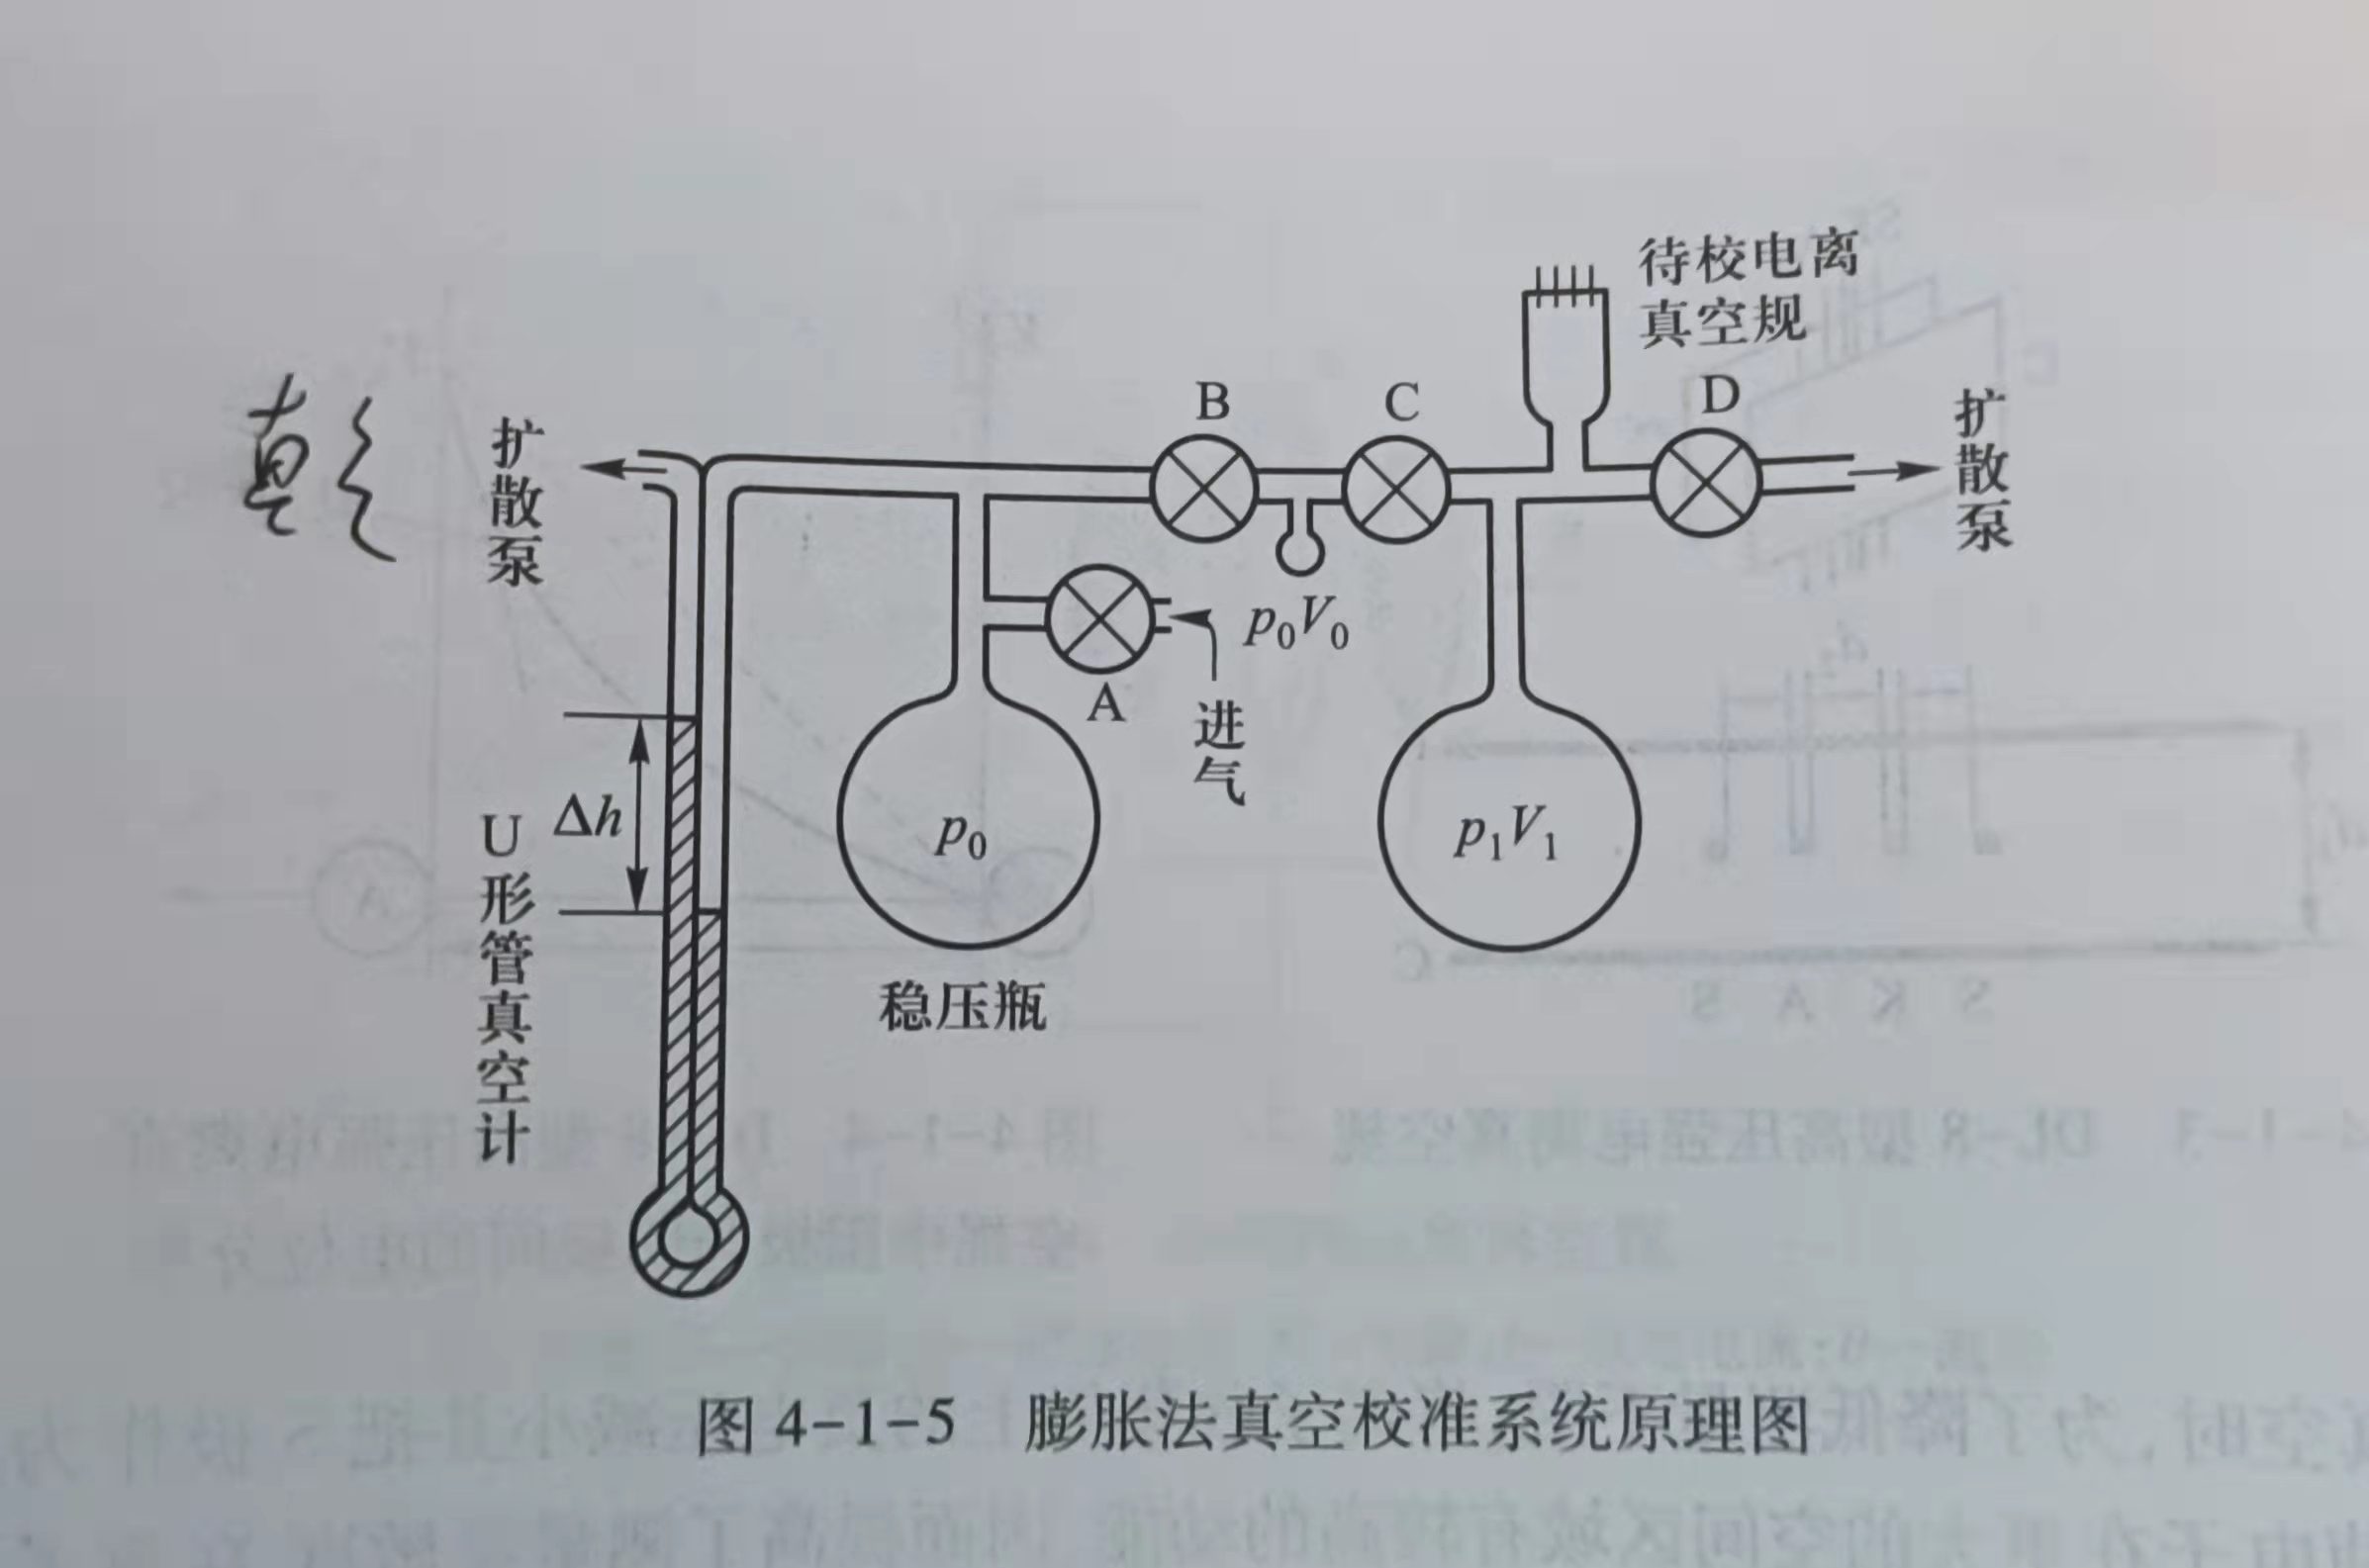
\includegraphics[height=10cm, width=14cm]{images/pic1.jpg}
 \label{fig:fig1}
\end{figure}
第一次膨胀有:
\begin{equation}
    p_1^{(1)}(V_0+V_1)=p_0V_0
\end{equation}
即
\begin{equation}
    p_1^{(1)}=\frac{V_0}{V_0+V_1}p_0
\end{equation}
第二次膨胀:
\begin{equation}
    p_1^{(2)}(V_0+V_1)=p_0V_0+p_1^{(1)}V_1
\end{equation}
即
\begin{equation}
    p_1^{(2)}=\frac{p_0V_0+p_1^{(1)}V_1}{V_0+V_1}
\end{equation}
类似地,对第n次膨胀有:
\begin{equation}
    p_1^{(n)}=\frac{p_0V_0+p_1^{(n-1)}V_1}{V_0+V_1}
\end{equation}
%%%%%%%%%%%%%%%%%%%%%%%%%%%%%%%%%%%%%%%% Experiment %%%%%%%%%%%%%%%%%%%%%%%%%%%%%%%%%%%%%%%%
\newpage
\section{实验} \label{experiment}%------------------------------

\subsection{实验仪器}\label{sub:sysover}
\begin{itemize}
\item{\textbf{U形管真空计}}
\item{\textbf{干燥瓶}}
\item{\textbf{机械泵}}
\item{\textbf{缓冲瓶}}
\item{\textbf{扩散泵}}
\item{\textbf{待校电离真空规}}

整个膨胀阀真空校准系统如下\textbf{图\ref{fig:fig2}}所示
\begin{figure}[H]
 \centering
 \caption{膨胀法真空校准系统图}
 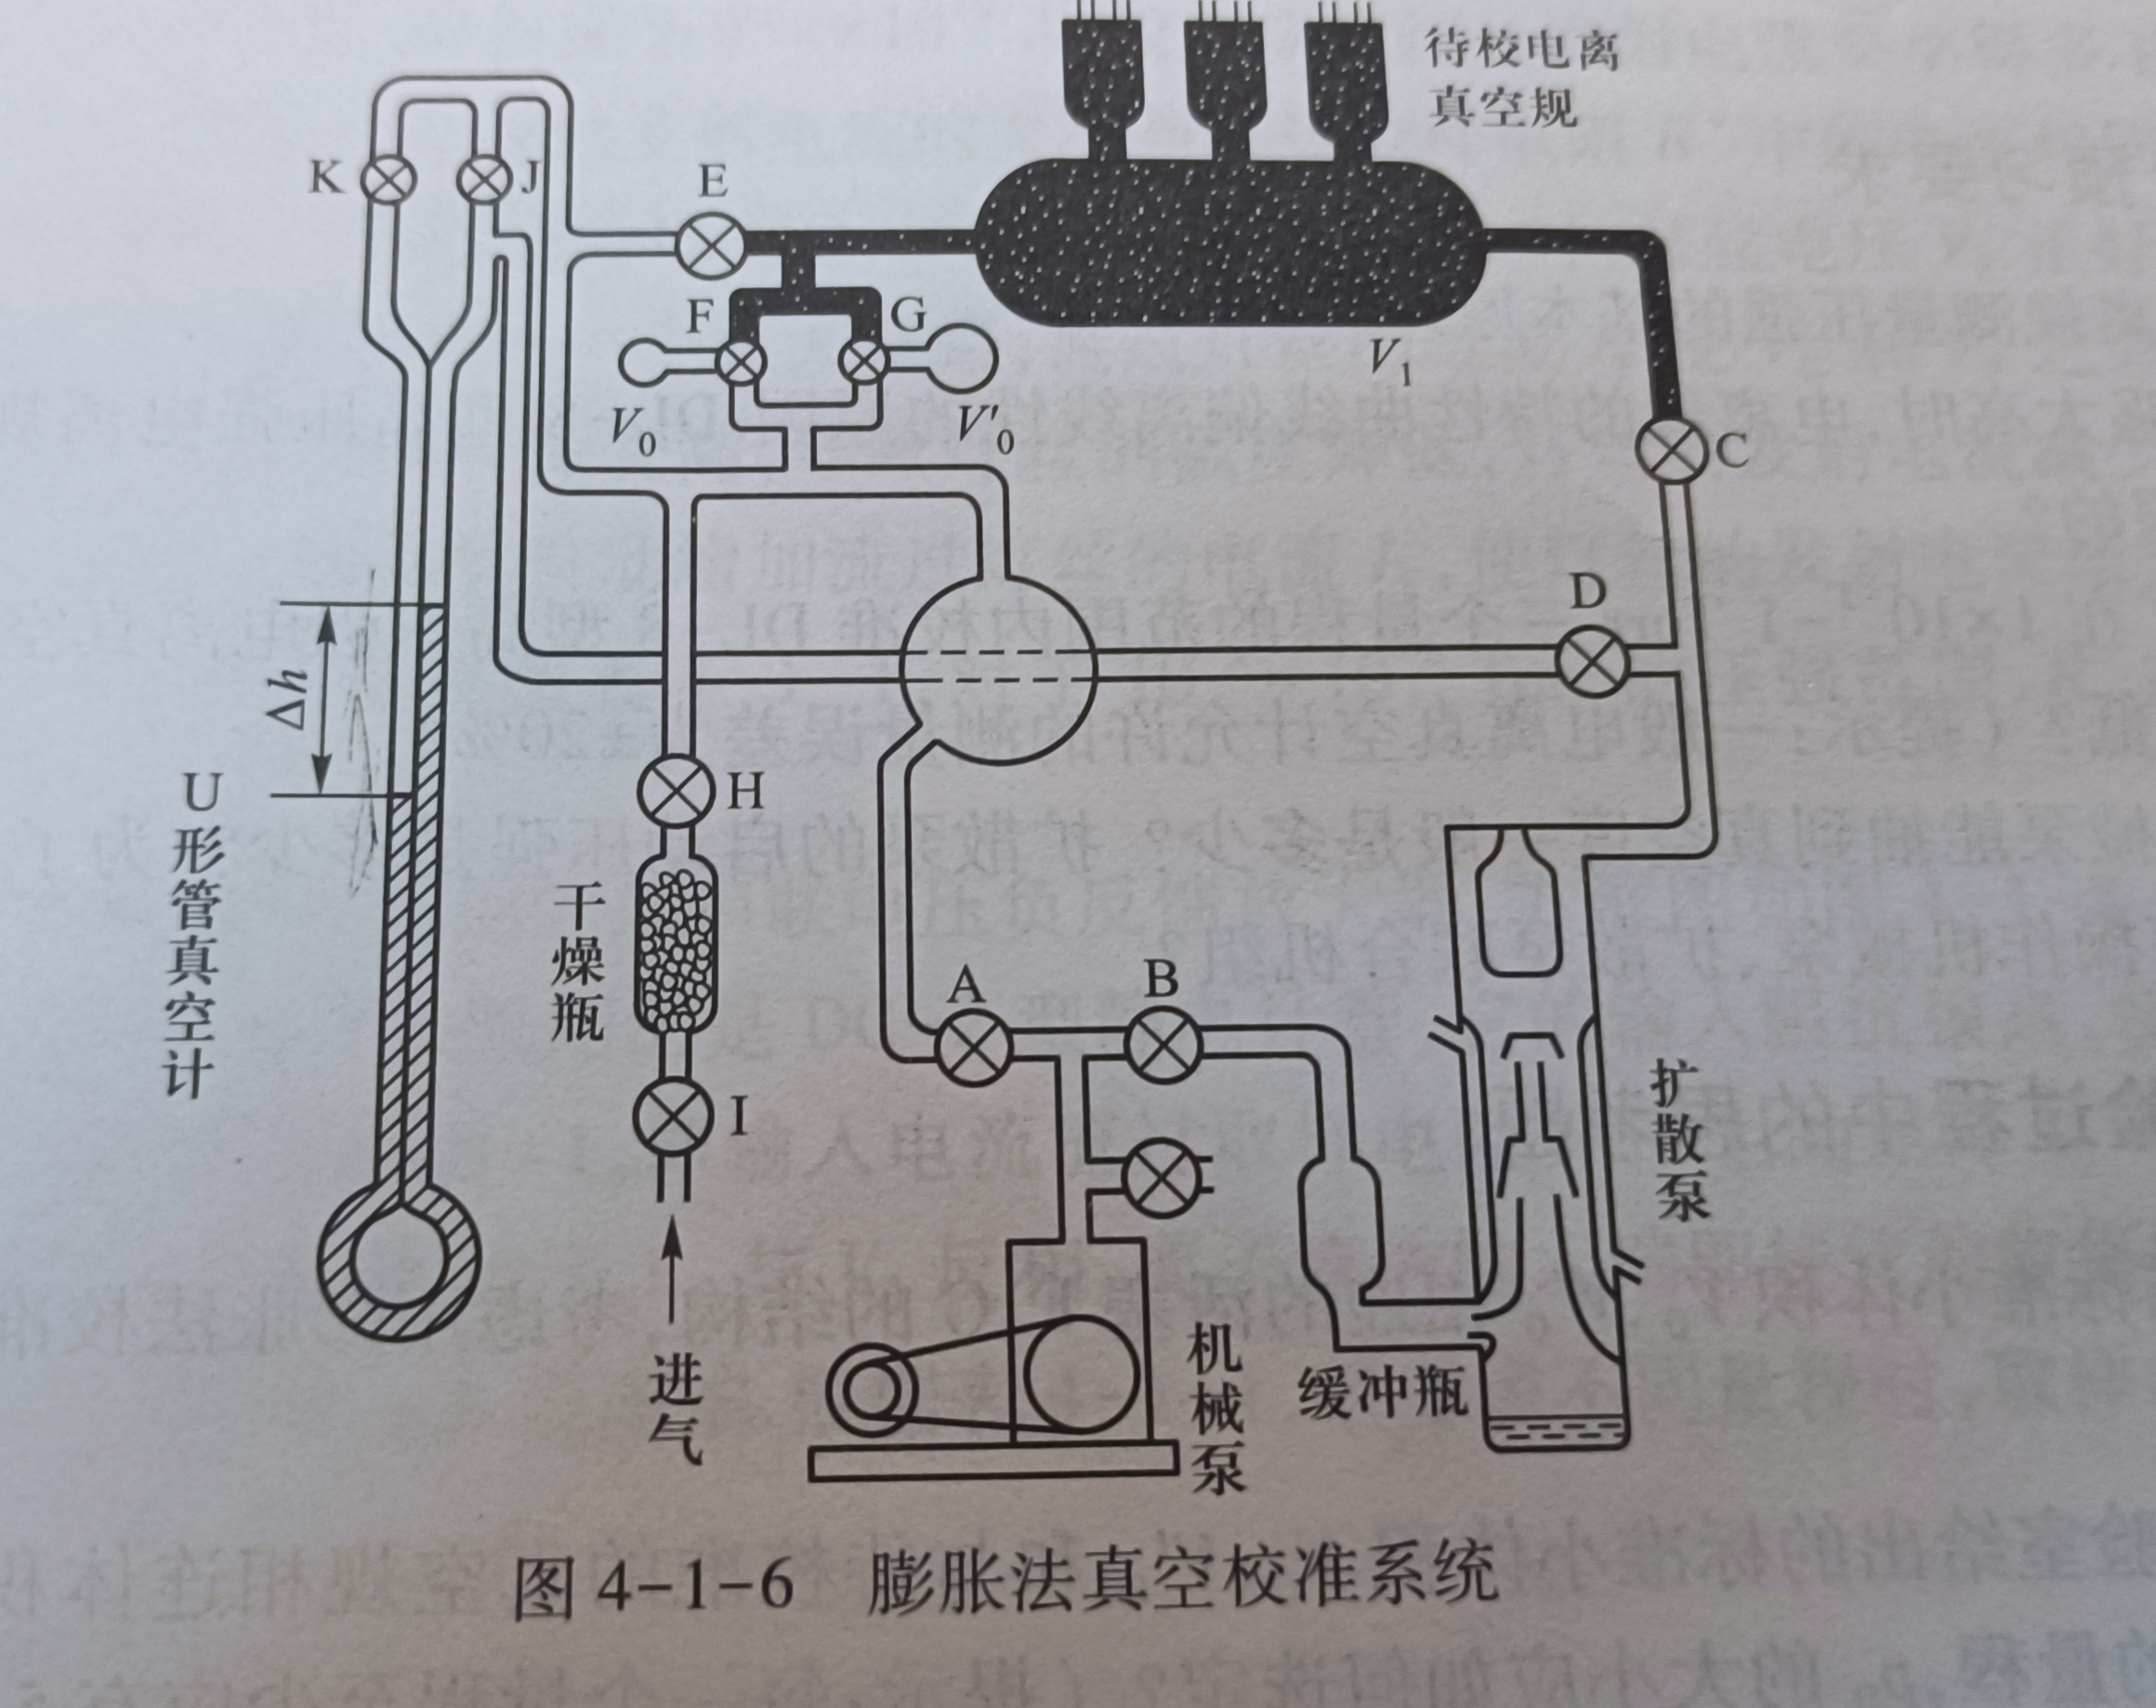
\includegraphics[height=10cm, width=14cm]{images/pic2.jpg}
 \label{fig:fig2}
\end{figure}
\end{itemize}
%------------------------------------------------------------
\begin{comment}
\newpage
\subsection{简要实验步骤}\label{sub:ExperimentalSteps}
分为以下几个步骤:\\\\
\circled{1}抽真空(按橘色按钮),约2分钟,机械泵声音平稳即可\\\\
\circled{2}整个系统抽至预备真空(约$10^{-2}~10^{-3}$Torr),然后,单对大体积$V_1$抽气,使$V_1$中的本底压强尽量低($<10^{-5}$Torr),必要时需用电吹风对这一部分进行烘烤\\\\
\circled{3}在真空状态下,将探测器放2$\sim$8号窗,分别测量能谱,记下活时间及能谱(最后转为文本文件以便分析),以便计算信号的计数率.等待的过程中进行蒙特卡洛模拟.\\\\
\circled{4}关掉真空泵按钮。在等待真空盒进入空气的过程中,利用$\gamma$源进行探测器刻度。\\\\
\circled{5}等真空表指示为0的时候,在真空盒充满空气状态下重复步骤3。等待的过程中进行蒙特卡洛模拟。比较同一位置空气及真空下的计数率,测量各窗能谱\\\\
\circled{6}进行能谱分析给出峰位,给出动量及动能关系图,写实验报告\\\\
\end{comment}

%%%%%%%%%%%%%%%%%%%%%%%%%%%%%%%%%%%%%%%% Results & Discussions %%%%%%%%%%%%%%%%%%%%%%%%%%%%%%%%%%%%%%%%
\newpage
\section{结果及讨论}
%------------------------------------------------------------
\subsection{关闭活塞C,用电离真空计测量$V_1$的本底压强随时间的变化.}\label{sub:1}
经过数据处理,我们可以得到如下\textbf{图\ref{fig:fig3}}所示结果 
\begin{figure}[H]
 \centering
 \caption{$V_1$的本底压强随时间的变化}
 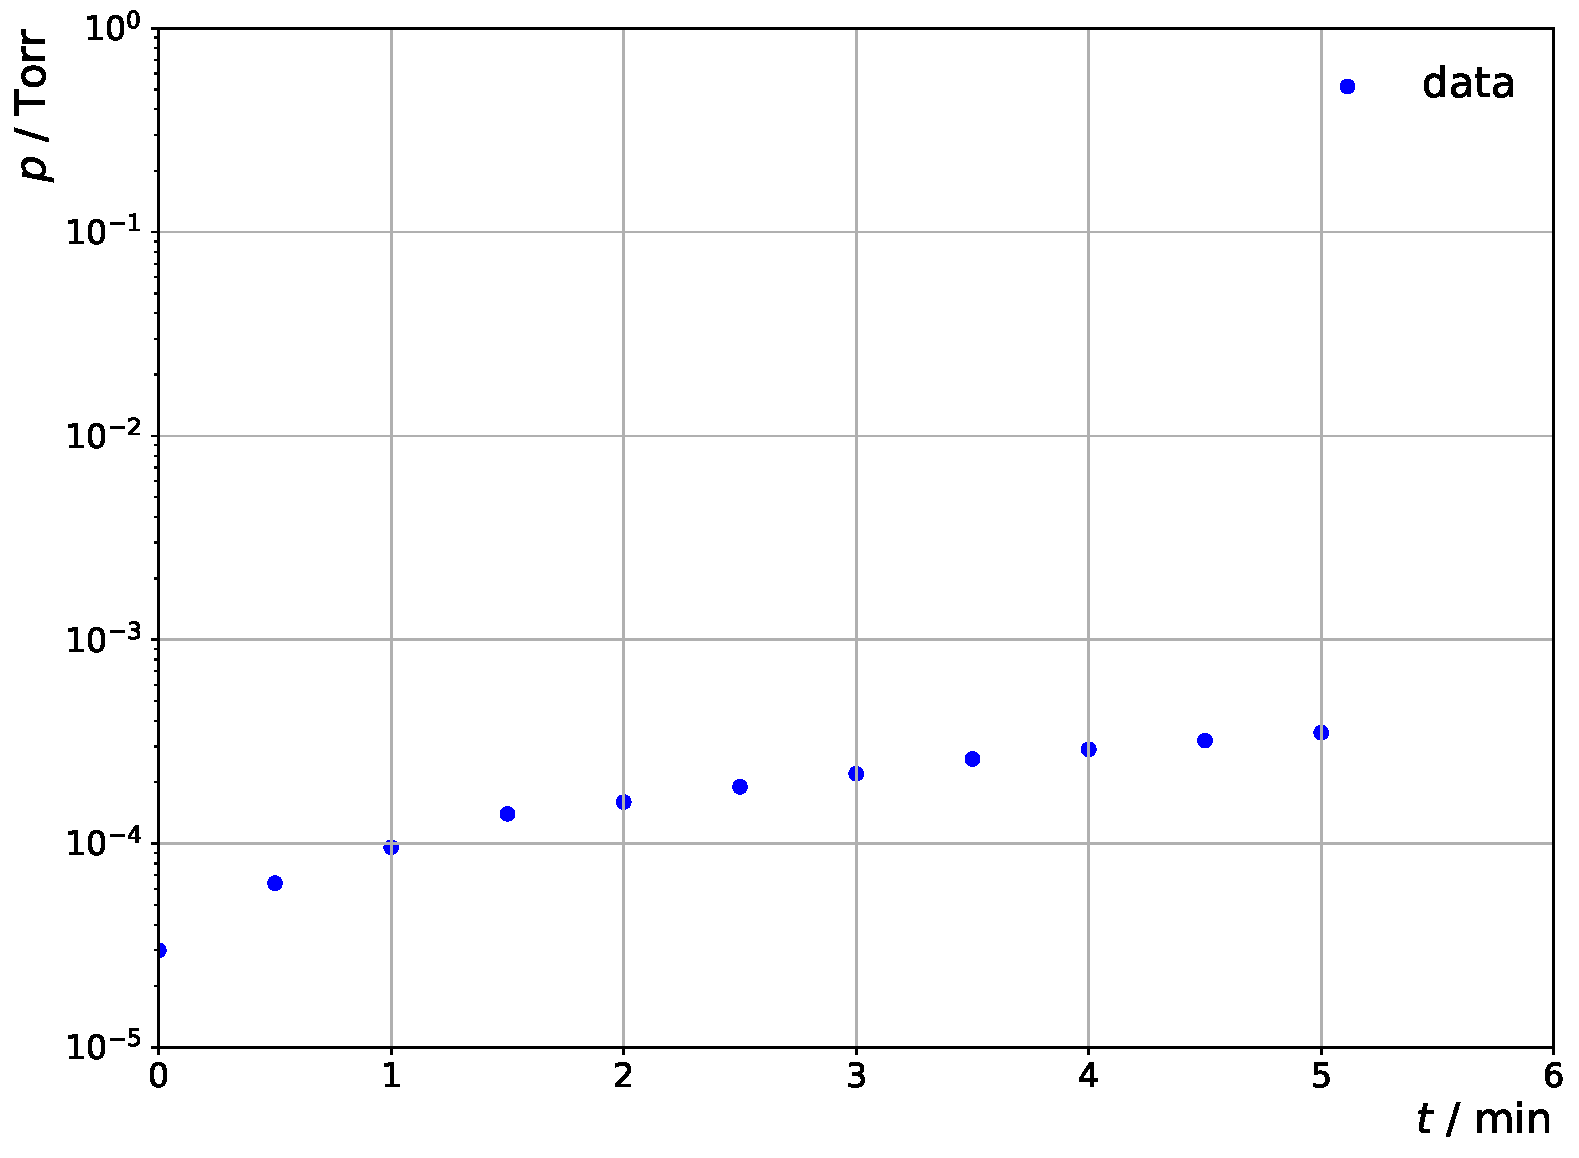
\includegraphics[height=12cm, width=16cm]{images/phyex1_fig1.pdf}
 \label{fig:fig3}
\end{figure}
显然可以得到本底压强的变化对真空计的校准影响较小,故可以忽略.\\
\begin{comment}
如果需要索引参考文献,请使用\cite{Erdos01}, 同时已经将参考文献的项目模版在文末写出。
\end{comment}
%------------------------------------------------------------
\subsection{用目测法求出U形管真空计两管中油面的高度差,求出稳压管中的压强$p_0$}\label{sub:2}
在$10^{-3}\sim10^{-2}$挡,U形管左边液面高度为$h_1=\SI{34.85}{cm}$,右边液面高度为$h_2=\SI{36.72}{cm}$,高度差为$\Delta h=\SI{1.87}{cm}$,压强为$p_0=\rho g\Delta h=\SI{1.50}{Torr}$

在$10^{-1}$挡,U形管左边液面高度为$h_1=\SI{28.30}{cm}$,右边液面高度为$h_2=\SI{43.50}{cm}$,高度差为$\Delta h=\SI{15.20}{cm}$,压强为$p_0=\rho g\Delta h=\SI{12.22}{Torr}$

%------------------------------------------------------------
\newpage
\subsection{电离真空计读数对应膨胀次数n的校准关系}\label{sub:3}
已知真空室体积为$V_1=2690mL$,小瓶体积为$V_0$,则每次膨胀后的压强为
\begin{equation}
    p_1^{(n)}=\frac{p_0V_0+p^{(n-1)}_1V_1}{V_0+V_1}
\end{equation}
\begin{enumerate}[1)]
    \item 对于$10^{-3}\si{Torr}$档的校准在膨胀次数为$n=0\sim n=9$阶段,小瓶体积$V_0=\SI{1.475}{mL}$,小瓶中初始压强$p_0=\SI{1.50}{Torr}$
    \item 对于$10^{-2}\si{Torr}$档的校准在膨胀次数为$n=10\sim n=32$阶段,小瓶体积$V_0=\SI{7.350}{mL}$,小瓶中初始压强$p_0=\SI{1.50}{Torr}$
    \item 对于$10^{-1}\si{Torr}$档的校准在膨胀次数为$n=33\sim n=59$阶段,小瓶体积$V_0=\SI{7.350}{mL}$,小瓶中初始压强$p_0=\SI{12.22}{Torr}$
\end{enumerate}
如下\textbf{图\ref{fig:fig4}}所示. 
\begin{figure}[H]
 \centering
 \caption{电离真空计读数对应膨胀次数n的校准关系}
 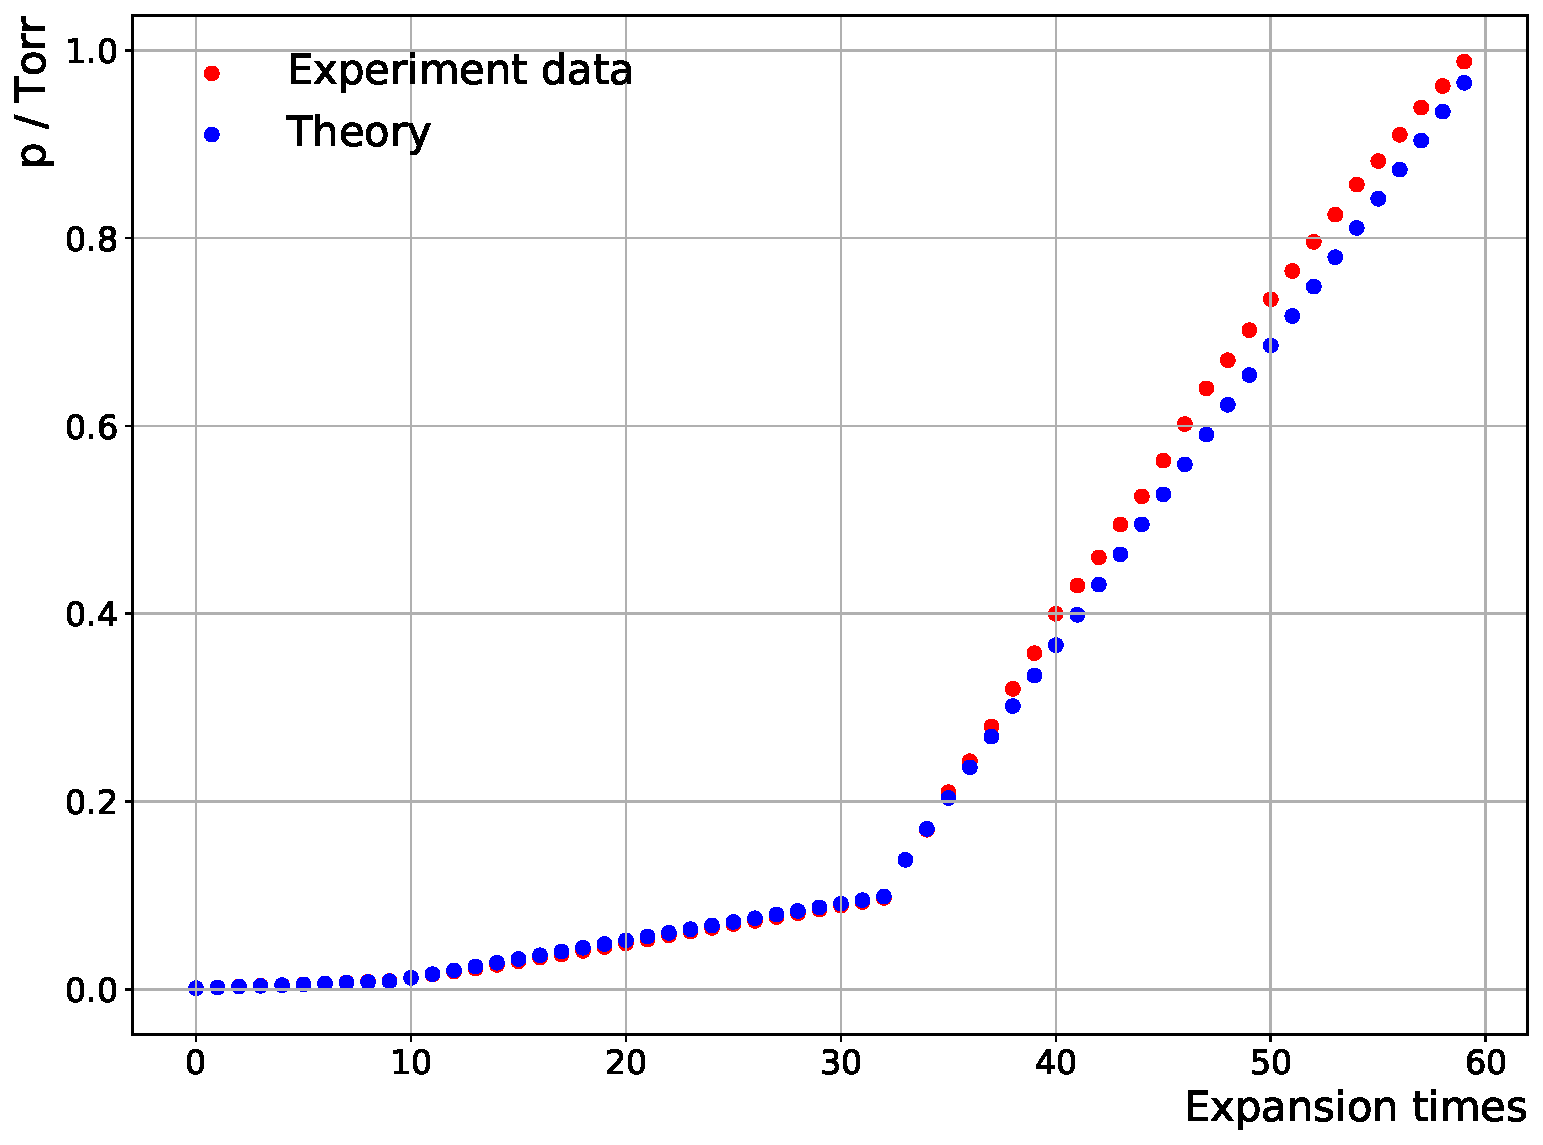
\includegraphics[height=12cm, width=16cm]{images/phyex1_fig2.pdf}
 \label{fig:fig4}
\end{figure}
值得注意的是,当我们切换到设置3)校准$10^{-3}\si{Torr}$档时,理论值$p_1$和实验中得到电离真空计读数偏差较大.
%------------------------------------------------------------
\newpage
\subsection{电离真空计读数与理论值的校准关系}\label{sub:4}

通过实验数据与理论预言曲线的比较,我们可以得到如下\textbf{图\ref{fig:fig5}}所结果. 
\begin{figure}[H]
 \centering
 \caption{真空和空气状态下测量得到动量动能关系与理论预言曲线比较}
 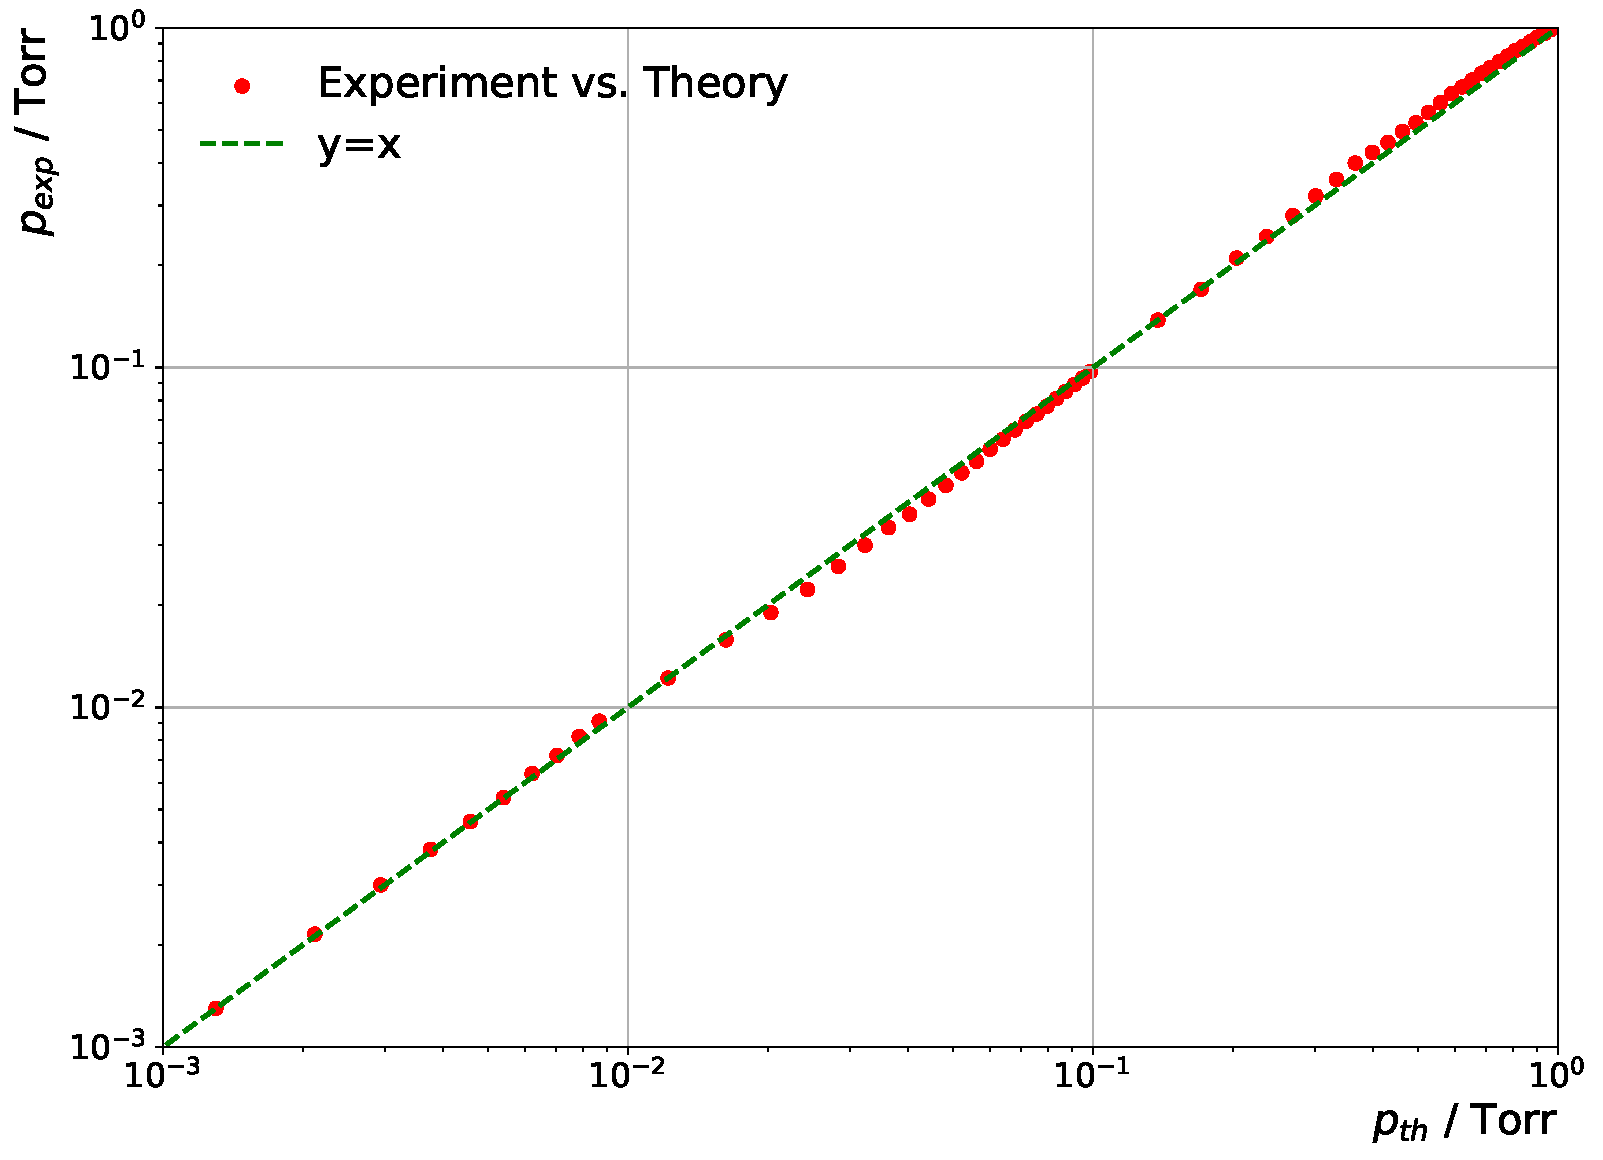
\includegraphics[height=12cm, width=16cm]{images/phyex1_fig3.pdf}
 \label{fig:fig5}
\end{figure}
\begin{enumerate}[1)]
    \item 可以看到,在$10^{-3}\si{Torr}$档线性关系符合较好.
    \item 在$10^{-2}\si{Torr}$档仪器读数整体低于标准值,可能是来源于我们切换小瓶体积$V_0$引入的误差.
    \item 而在$10^{-1}\si{Torr}$档仪器读数整体高于标准值,可能是来源于我们为了适应该单位而改变液面高度差$\Delta h$引入的误差.
\end{enumerate}






通过数据分析可得最大相对误差为$\delta_{max}=9.1\%$,满足精度小于$10\%$的要求.

%add more subsections for other block
%%%%%%%%%%%%%%%%%%%%%%%%%%%%%%%%%%%%%%%% Conclusion %%%%%%%%%%%%%%%%%%%%%%%%%%%%%%%%%%%%%%%%
\newpage
\section{结论}\label{conclusions}
本实验利用膨胀法校准了高压强电离真空计,同时还利用实验室提高的辅助教学软件研究了DL-8型电离规内的电场分布及电子轨迹.

探究了电离规测量压强的基本原理,测量了仪器的最大相对误差,符合10\%的精度要求,对电离规的特性曲线偏离线性的原因给予了一定的解释.

%%%%%%%%%%%%%%%%%%%%%%%%%%%%%%%%%%%%%%%% Questions %%%%%%%%%%%%%%%%%%%%%%%%%%%%%%%%%%%%%%%%
\begin{comment}
\section{实验报告思考题}\label{questions}
\subsection{在$a=23.0mm$、$b=10.0mm$的矩形波导管中能不能传播$\lambda=2cm$、$3cm$和$5cm$的微波?各能传播哪些波型?}\label{sub:question1}
答:根据
\begin{equation}
    \lambda_c=\frac{2}{\sqrt{(m/a)^2+(n/b)^2}}
\end{equation}
我们可以算出可传播的最大波长为$\lambda_{max}=18.3mm$,显然不能传播$\lambda=2cm$、$3cm$和$5cm$的微波,可传输波长在$\lambda_{max}=18.3mm$以下,满足$\lambda_c=\frac{2}{\sqrt{(m/a)^2+(n/b)^2}}$的波长的波型\\

\end{comment}

%%%%%%%%%%%%%%%%%%%%%%%%%%%%%%%%%%%%%%%% Acknowledgements %%%%%%%%%%%%%%%%%%%%%%%%%%%%%%%%%%%%%%%%

\section{致谢}\label{acknowledgments}
感谢老师在实验中的的悉心指导.

\begin{comment}
%%%%%%%%%%%%%%%%%%%%%%%%%%%%%%%%%%%%%%%% Appendix %%%%%%%%%%%%%%%%%%%%%%%%%%%%%%%%%%%%%%%%
\appendix
\section{代码}\label{sub:app.code}
请在附录\ref{sub:app.code}中添加代码。请使用如下Scala的语法高亮描述方法。
\begin{scala}
class TopIO extends Bundle() {
	val boot = Input(Bool()) 
// imem and dmem interface for Tests
	val test_im_wr		= Input(Bool())
	val test_im_rd 		= Input(Bool())
	val test_im_addr 	= Input(UInt(32.W))
	val test_im_in 		= Input(UInt(32.W))
	val test_im_out 	= Output(UInt(32.W))

	val test_dm_wr		= Input(Bool())
	val test_dm_rd 		= Input(Bool())
	val test_dm_addr 	= Input(UInt(32.W))
	val test_dm_in 		= Input(UInt(32.W))
	val test_dm_out 	= Output(UInt(32.W))

	val valid			= Output(Bool())
}
class Top extends Module() {
	val io 		= IO(new TopIO())//in chisel3, io must be wrapped in IO(...) 
	//...
	when (io.boot & io.test_im_wr){
		imm(io.test_im_addr) := io.test_im_in
		} .elsewhen (io.boot & io.test_dm_wr){
		// please finish it
		} //...
}
\end{scala}
\newpage

%%%%%%%%%%%%%%%%%%%%%%%%%%%%%%%%%%%%%%%% REFERENCE %%%%%%%%%%%%%%%%%%%%%%%%%%%%%%%%%%%%%%%%
\begin{thebibliography}{9}

\bibitem{Erdos01} P. Erd\H os, \emph{A selection of problems and
results in combinatorics}, Recent trends in combinatorics (Matrahaza,
1995), Cambridge Univ. Press, Cambridge, 2001, pp. 1--6.

\end{thebibliography}
\end{comment}
\end{document}

